
% libmusicxml2 architecture overview
% Grame, 2020

%\documentclass[border=20pt]{standalone}
\documentclass[12pt,a4paper]{article}

% -------------------------------------------------------------------------
% import common LaTeX settings
% -------------------------------------------------------------------------

\usepackage{import}

\subimport{../}{CommonLaTeXSettings}

\usepackage{tikz}

\usetikzlibrary{math}
%\usetikzlibrary{arrows.meta}

\usepackage{changepage} % for adjustwidth


% -------------------------------------------------------------------------
\begin{document}
% -------------------------------------------------------------------------

\title{
\lib\ architecture overview \\[5pt]
{\normalsize 
  \xmlToGuido\ v2.3, \xmlToLy\ v0.9, \xmlToBrl\ v0.01\\
  \today
}
}

%\author{
%Jacques Menu 
%}

%\date {(as of \normalsize \today)}
\date {}

\maketitle
\thispagestyle{fancy} % right after \maketitle to apply it to the first page too


%\tableofcontents

This document shows the architecture of the \lib\ library, to be found at 
\url {https://github.com/grame-cncm/libmusicxml/tree/lilypond}.

\lib\ is written in C++11 and provides a set of music scores representations and converters between various textual music scores formats. Building it only requires a C++11 compiler and {\tt cmake}.


% -------------------------------------------------------------------------
\section{Architecture}
% -------------------------------------------------------------------------

The picture at figure \ref {Architecture}, page \pageref {Architecture}, shows how \lib\ is structured. The dimmed, dashed arrows indicate items not yet available. 
The numbered arrows show the existing conversions between formats and representations.

\begin{adjustwidth}{-1cm}{-1cm}
\begin{figure}[h]
\caption {\lib\ architecture}
\label{Architecture}
\begin{center}

% -------------------------------------------------------------------------
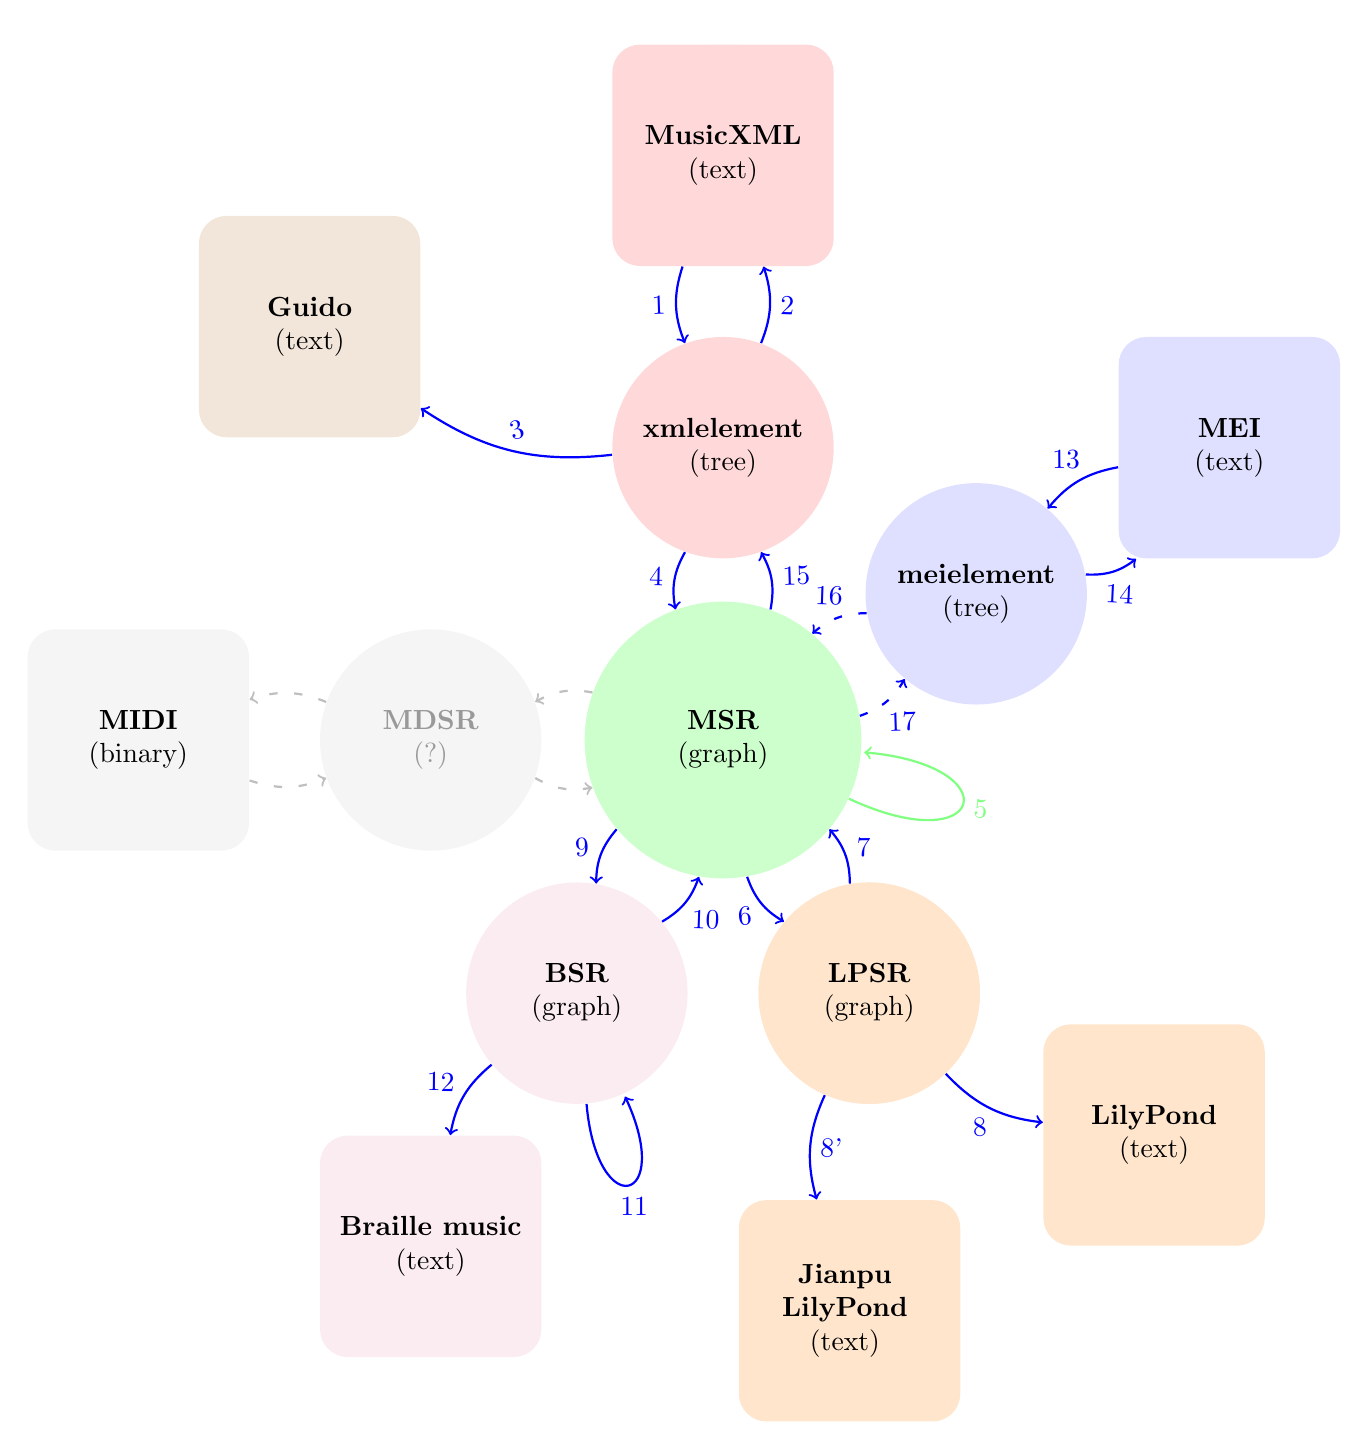
\begin{tikzpicture}[scale=0.675] % allow upside down ???
% -------------------------------------------------------------------------

% elements positions
% ------------------------------------------------

\tikzmath{
	% dilatation factor
	\interalDiameter = 5.5;
	%
	% diameters ration
	\externalDiameter = 11;
	%
  % MSR
  \MSRAbs = 0;
  \MSROrd = 0;
  %
  % UpperSpace
  \UpperSpaceAbs = 0;
  \UpperSpaceOrd = \externalDiameter * 1.1;
	%
  % MusicXMLTree
  \MusicXMLTreeAngle = 90;
  \MusicXMLTreeAbs = \interalDiameter*cos(\MusicXMLTreeAngle);
  \MusicXMLTreeOrd = \interalDiameter*sin(\MusicXMLTreeAngle);
  %
  % MusicXML
  \MusicXMLAngle = \MusicXMLTreeAngle;
  \MusicXMLAbs = \externalDiameter*cos(\MusicXMLAngle);
  \MusicXMLOrd = \externalDiameter*sin(\MusicXMLAngle);
  %
  % Guido
  \GuidoAngle = 135;
  \GuidoAbs = \externalDiameter*cos(\GuidoAngle);
  \GuidoOrd = \externalDiameter*sin(\GuidoAngle);
  %
  % MEITree
  \MEITreeAngle = 30;
  \MEITreeAbs = \interalDiameter*cos(\MEITreeAngle);
  \MEITreeOrd = \interalDiameter*sin(\MEITreeAngle);
  %
  % MEI
  \MEIAngle = \MEITreeAngle;
  \MEIAbs = \externalDiameter*cos(\MEIAngle);
  \MEIOrd = \externalDiameter*sin(\MEIAngle);
  %
  % MDSR
  \MDSRAngle = 180;
  \MDSRAbs = \interalDiameter*cos(\MDSRAngle);
  \MDSROrd = \interalDiameter*sin(\MDSRAngle);
  %
  % MIDI
  \MIDIAngle = \MDSRAngle;
  \MIDIAbs      = \externalDiameter*cos(\MIDIAngle);
  \MIDIOrd      = \externalDiameter*sin(\MIDIAngle);
  %
  % LPSR
  \LPSRAngle = 300;
  \LPSRAbs      = \interalDiameter*cos(\LPSRAngle);
  \LPSROrd      = \interalDiameter*sin(\LPSRAngle);
  %
  % LilyPond
  \LilyPondAngle = \LPSRAngle + 17.5;
  \LilyPondAbs   = \externalDiameter*cos(\LilyPondAngle);
  \LilyPondOrd   = \externalDiameter*sin(\LilyPondAngle);
  %
  % Jianpu LilyPond
  \JianpuLilyPondAngle = \LPSRAngle - 17.5;
  \JianpuLilyPondAbs   = \externalDiameter*cos(\JianpuLilyPondAngle);
  \JianpuLilyPondOrd   = \externalDiameter*sin(\JianpuLilyPondAngle);
  %
  % BSR
  \BSRAngle = 240;
  \BSRAbs      = \interalDiameter*cos(\BSRAngle);
  \BSROrd      = \interalDiameter*sin(\BSRAngle);
  %
  % BrailleMusic
  \BrailleMusicAngle = \BSRAngle;
  \BrailleMusicAbs   = \externalDiameter*cos(\BrailleMusicAngle);
  \BrailleMusicOrd   = \externalDiameter*sin(\BrailleMusicAngle);
  %
  % RandomMusic
  \RandomMusicStartAbs = -1.55;
  \RandomMusicStartOrd = \MusicXMLTreeOrd + 0.35;
  \RandomMusicInterAbs = \MusicXMLTreeAbs - 0.10;
  \RandomMusicInterOrd = \MusicXMLTreeOrd - 0.10;
  \RandomMusicEndAbs   = \MusicXMLAbs - 0.20;
  \RandomMusicEndOrd   = \MusicXMLOrd - 0.15;
  %
  % textOutput
  \textOutputAngle = 135;
  \textOutputRadius = 1.6;
  \textOutputAbs = cos(\textOutputAngle) * \textOutputRadius;
  \textOutputOrd = sin(\textOutputAngle) * \textOutputRadius;
  %
  % tools
  \toolsStartAbs = \MusicXMLAbs - 0.125;
  \toolsStartOrd = \MusicXMLOrd - 0.15;
  \toolsInterAbs = \MusicXMLTreeAbs - 0.05;
  \toolsInterOrd = \MusicXMLTreeOrd - 0.1;
  \toolsEndAbs   = \textOutputAbs + 0.15;
  \toolsEndOrd   = \textOutputOrd + 0.0;
  %
  % xmlToGuido
  \xmlToGuidoInterangle = (\MusicXMLTreeAngle + \GuidoAngle) / 2;
  \xmlToGuidoInterRadius = 0.6;
  \xmlToGuidoStartAbs = \MusicXMLAbs + 0.15;
  \xmlToGuidoStartOrd = \MusicXMLOrd - 0.15;
  \xmlToGuidoInterAbs = cos(\xmlToGuidoInterangle) * \xmlToGuidoInterRadius;
  \xmlToGuidoInterOrd = sin(\xmlToGuidoInterangle) * \xmlToGuidoInterRadius;
  \xmlToGuidoEndAbs   = \GuidoAbs - 0.15;
  \xmlToGuidoEndOrd   = \GuidoOrd - 0.15;
  %
  % xml2ly
  \xmlToLyInterIAngle  = mod((\MusicXMLTreeAngle + \LPSRAngle) * 2 / 3, 360);
  \xmlToLyInterIIAngle = mod((\MusicXMLTreeAngle + \LPSRAngle) * 1 / 3, 360);
  \xmlToLyInterRadius = 0.10;
  \xmlToLyStartAbs = \MusicXMLAbs + 0.05;
  \xmlToLyStartOrd = \MusicXMLOrd - 0.15;
  \xmlToLyInterIAbs = cos(\xmlToLyInterIAngle) * \xmlToLyInterRadius;
  \xmlToLyInterIOrd = sin(\xmlToLyInterIAngle) * \xmlToLyInterRadius;
  \xmlToLyInterIIAbs = cos(\xmlToLyInterIIAngle) * \xmlToLyInterRadius;
  \xmlToLyInterIIOrd = sin(\xmlToLyInterIIAngle) * \xmlToLyInterRadius;
  \xmlToLyEndAbs   = \LilyPondAbs - 0.045;
  \xmlToLyEndOrd   = \LilyPondOrd + 0.15;
  %
  % xml2brl
  \xmlToBrlInterIAngle  = mod((\MusicXMLTreeAngle + \LPSRAngle) * 2 / 3, 360);
  \xmlToBrlInterIIAngle = mod((\MusicXMLTreeAngle + \LPSRAngle) * 1 / 3, 360);
  \xmlToBrlInterRadius = 0.2;
  \xmlToBrlStartAbs = \MusicXMLAbs + 0.10;
  \xmlToBrlStartOrd = \MusicXMLOrd - 0.15;
  \xmlToBrlInterIAbs = cos(\xmlToBrlInterIAngle) * \xmlToBrlInterRadius;
  \xmlToBrlInterIOrd = sin(\xmlToBrlInterIAngle) * \xmlToBrlInterRadius;
  \xmlToBrlInterIIAbs = cos(\xmlToBrlInterIIAngle) * \xmlToBrlInterRadius;
  \xmlToBrlInterIIOrd = sin(\xmlToBrlInterIIAngle) * \xmlToBrlInterRadius;
  \xmlToBrlEndAbs   = \BrailleMusicAbs - 0.05;
  \xmlToBrlEndOrd   = \BrailleMusicOrd + 0.15;
  %
  % toBeWrittenCommon
  \toBeWrittenCommonStartAbs = -1.15;
  \toBeWrittenCommonStartOrd = \MDSROrd + 0.65;
  \toBeWrittenCommonEndAbs = \toBeWrittenCommonStartAbs + 0.65;
  \toBeWrittenCommonEndOrd = \toBeWrittenCommonStartOrd - 0.225;
  %
  % toBeWrittenToMusicXML
  \toBeWrittenToMusicXMLInterIAngle  = mod((\MusicXMLTreeAngle + \MDSRAngle) * -0.1, 360);
  \toBeWrittenToMusicXMLInterIIAngle = mod((\MusicXMLTreeAngle + \MDSRAngle) * 0.375, 360);
  \toBeWrittenToMusicXMLInterRadius = -0.20;
  \toBeWrittenToMusicXMLStartAbs = \toBeWrittenCommonEndAbs;
  \toBeWrittenToMusicXMLStartOrd = \toBeWrittenCommonEndOrd;
  \toBeWrittenToMusicXMLInterIAbs = cos(\toBeWrittenToMusicXMLInterIAngle) * \toBeWrittenToMusicXMLInterRadius;
  \toBeWrittenToMusicXMLInterIOrd = sin(\toBeWrittenToMusicXMLInterIAngle) * \toBeWrittenToMusicXMLInterRadius;
  \toBeWrittenToMusicXMLInterIIAbs = cos(\toBeWrittenToMusicXMLInterIIAngle) * \toBeWrittenToMusicXMLInterRadius;
  \toBeWrittenToMusicXMLInterIIOrd = sin(\toBeWrittenToMusicXMLInterIIAngle) * \toBeWrittenToMusicXMLInterRadius;
  \toBeWrittenToMusicXMLEndAbs   = \MusicXMLAbs - 0.05;
  \toBeWrittenToMusicXMLEndOrd   = \MusicXMLOrd - 0.15;
	%
  % toBeWrittenToLilyPond
  \toBeWrittenToLilyPondInterIAngle  = mod((\LPSRAngle + \MDSRAngle) * -0.1, 360);
  \toBeWrittenToLilyPondInterIIAngle = mod((\LPSRAngle + \MDSRAngle) * 0.375, 360);
  \toBeWrittenToLilyPondInterRadius = 0.30;
  \toBeWrittenToLilyPondStartAbs = \toBeWrittenCommonEndAbs5;
  \toBeWrittenToLilyPondStartOrd = \toBeWrittenCommonEndOrd;
  \toBeWrittenToLilyPondInterIAbs = cos(\toBeWrittenToLilyPondInterIAngle) * \toBeWrittenToLilyPondInterRadius;
  \toBeWrittenToLilyPondInterIOrd = sin(\toBeWrittenToLilyPondInterIAngle) * \toBeWrittenToLilyPondInterRadius;
  \toBeWrittenToLilyPondInterIIAbs = cos(\toBeWrittenToLilyPondInterIIAngle) * \toBeWrittenToLilyPondInterRadius;
  \toBeWrittenToLilyPondInterIIOrd = sin(\toBeWrittenToLilyPondInterIIAngle) * \toBeWrittenToLilyPondInterRadius;
  \toBeWrittenToLilyPondEndAbs   = \LilyPondAbs - 0.15;
  \toBeWrittenToLilyPondEndOrd   = \LilyPondOrd - 0.15;
	%
  % toBeWrittenToBrailleMusic
  \toBeWrittenToBrailleMusicInterIAngle  = mod((\LPSRAngle + \MDSRAngle) * -0.1, 360);
  \toBeWrittenToBrailleMusicInterIIAngle = mod((\LPSRAngle + \MDSRAngle) * 0.375, 360);
  \toBeWrittenToBrailleMusicInterRadius = 0.30;
  \toBeWrittenToBrailleMusicStartAbs = \toBeWrittenCommonEndAbs5;
  \toBeWrittenToBrailleMusicStartOrd = \toBeWrittenCommonEndOrd;
  \toBeWrittenToBrailleMusicInterIAbs = cos(\toBeWrittenToBrailleMusicInterIAngle) * \toBeWrittenToBrailleMusicInterRadius;
  \toBeWrittenToBrailleMusicInterIOrd = sin(\toBeWrittenToBrailleMusicInterIAngle) * \toBeWrittenToBrailleMusicInterRadius;
  \toBeWrittenToBrailleMusicInterIIAbs = cos(\toBeWrittenToBrailleMusicInterIIAngle) * \toBeWrittenToBrailleMusicInterRadius;
  \toBeWrittenToBrailleMusicInterIIOrd = sin(\toBeWrittenToBrailleMusicInterIIAngle) * \toBeWrittenToBrailleMusicInterRadius;
  \toBeWrittenToBrailleMusicEndAbs   = \BrailleMusicAbs - 0.15;
  \toBeWrittenToBrailleMusicEndOrd   = \BrailleMusicOrd - 0.15;
  %
%  % title
%  \titleAbs = -1.2;
%  \titleOrd = 3.0;
%  %
%  % table
%  \tableOrd = -2.8;
%  %
%  % bottom line
%  \bottomLineOrd = -3.5;
%  %
%  % legend
%  \legendAbs = -2.3;
%  \legendOrd = -3.4;
%  %
%  % date
%  \dateAbs = 0.25;
%  \dateOrd = \bottomLineOrd-0.2;
}


% The coordinates
% ------------------------------------------------

\coordinate (MSR) at (\MSRAbs,\MSROrd);

\coordinate (UpperSpace) at (\UpperSpaceAbs,\UpperSpaceOrd);

\coordinate (MusicXMLTree) at (\MusicXMLTreeAbs,\MusicXMLTreeOrd);
\coordinate (MusicXML) at (\MusicXMLAbs,\MusicXMLOrd);

\coordinate (Guido) at (\GuidoAbs,\GuidoOrd);

\coordinate (LPSR) at (\LPSRAbs, \LPSROrd);
\coordinate (LilyPond) at (\LilyPondAbs, \LilyPondOrd);
\coordinate (JianpuLilyPond) at (\JianpuLilyPondAbs, \JianpuLilyPondOrd);

\coordinate (BrailleMusic) at (\BrailleMusicAbs, \BrailleMusicOrd);
\coordinate (BSR) at (\BSRAbs, \BSROrd);

\coordinate (MEITree) at (\MEITreeAbs,\MEITreeOrd);
\coordinate (MEI) at (\MEIAbs,\MEIOrd);

\coordinate (MIDI) at (\MIDIAbs, \MIDIOrd);
\coordinate (MDSR) at (\MDSRAbs, \MDSROrd);

\coordinate (textOutput) at (\textOutputAbs, \textOutputOrd);


% Draw the elements
% ------------------------------------------------

\def \minimumCircelSize {80}

\def \MusicXMLColor {red!15}

\def \GuidoColor {brown!20}

\def \LilyPondColor {orange!20}

\def \BrailleMusicColor {purple!7.5}

\def \MEIColor {blue!12.5}

\def \MIDIColor {black!3.75}

\def \roundedCorners {10pt}

% MSR
\node[align=center,style={circle,minimum size=100,fill=green!20}]
  (MSR) at (MSR) {{\bf MSR}\\(graph)};

% UpperSpace
\node[align=center,style={rectangle,minimum height=50,fill=white}]
  (UpperSpace) at (UpperSpace) {~};

% MusicXML
\node[align=center,style={rectangle,rounded corners=\roundedCorners,minimum size=\minimumCircelSize,fill=\MusicXMLColor}]
  (MusicXML)
  at (MusicXML) {{\bf MusicXML}\\(text)};

% MusicXMLTree
\node[align=center,style={circle,minimum size=\minimumCircelSize,fill=\MusicXMLColor}]
  (MusicXMLTree)
  at (MusicXMLTree) {{\bf xmlelement}\\(tree)};
  
% Guido
\node[align=center,style={rectangle,rounded corners=\roundedCorners,minimum size=\minimumCircelSize,fill=\GuidoColor}]
  (Guido) at (Guido) {{\bf Guido}\\(text)};
 
% MEI
\node[align=center,style={rectangle,rounded corners=\roundedCorners,minimum size=\minimumCircelSize,fill=\MEIColor}]
  (MEI) at (MEI) {{\bf MEI}\\(text)};
 
% MEITree
\node[align=center,style={circle,minimum size=\minimumCircelSize,fill=\MEIColor}]
  (MEITree)
  at (MEITree) {{\bf meielement}\\(tree)};
  
% LilyPond
\node[align=center,style={rectangle,rounded corners=\roundedCorners,minimum size=\minimumCircelSize,fill=\LilyPondColor}]
  (LilyPond)
  at (LilyPond) {{\bf LilyPond}\\(text)};
\node[align=center,style={circle,minimum size=\minimumCircelSize,fill=\LilyPondColor}]
  (LPSR)
  at (LPSR) {{\bf LPSR}\\(graph)};

% Jianpu LilyPond
\node[align=center,style={rectangle,rounded corners=\roundedCorners,minimum size=\minimumCircelSize,fill=\LilyPondColor}]
  (JianpuLilyPond)
  at (JianpuLilyPond) {
    \parbox [c] {1.8cm} {
    	\centering {\bf Jianpu}
			\\
			\centering {\bf LilyPond}
			\\
			\centering {(text)}
    }
  };
\node[align=center,style={circle,minimum size=\minimumCircelSize,fill=\LilyPondColor}]
  (LPSR)
  at (LPSR) {{\bf LPSR}\\(graph)};

% BrailleMusic
\node[align=center,style={rectangle,rounded corners=\roundedCorners,minimum size=\minimumCircelSize,fill=\BrailleMusicColor}]
  (BrailleMusic)
  at (BrailleMusic) {{\bf Braille music}\\(text)};
\node[align=center,style={circle,minimum size=\minimumCircelSize,fill=\BrailleMusicColor}]
  (BSR)
  at (BSR) {{\bf BSR}\\(graph)};

% MIDI
\node[align=center,style={rectangle,rounded corners=\roundedCorners,minimum size=\minimumCircelSize,fill=\MIDIColor}]
  (MIDI)
  at (MIDI) {{\bf MIDI}\\(binary)};
  
% MDSR
\node[align=center,style={circle,minimum size=\minimumCircelSize,fill=\MIDIColor,text=gray!\minimumCircelSize}]
  (MDSR)
  at (MDSR) {{\bf MDSR}\\(?)};

%% textOutput
%\node[align=center]
%  (textOutput)
%  at (textOutput) {\includegraphics[scale=0.15]{TextOutputIcon.png}};


% Draw the arcs between the elements
% ------------------------------------------------

\def \bendAngle {20}

\def \arcsColor {blue}
\def \dashedArcsColor {gray!50}
\def \implicitColor {green!50}

% MusicXML <-> MusicXMLTree
\path [->, sloped, bend right=\bendAngle, below, thick, \arcsColor] 
(MusicXML) 
edge node {\rotatebox{90}{1}} 
(MusicXMLTree);

\path [->, sloped, bend right=\bendAngle, below, thick, \arcsColor] 
(MusicXMLTree) 
edge node {\rotatebox{-90}{2}} 
(MusicXML);

% MusicXMLTree -> Guido
\path [->, sloped, bend left=\bendAngle, above, thick, \arcsColor] 
(MusicXMLTree) 
edge node {\rotatebox{30}{3}} 
(Guido);

% MusicXMLTree <-> MSR
\path [->, sloped, bend right=\bendAngle, above, thick, \arcsColor] 
(MusicXMLTree) 
edge node {\rotatebox{-82}{4}} 
(MSR);

\path [->, sloped, bend right=\bendAngle, above, thick, \arcsColor] 
(MSR) 
edge node {\rotatebox{82.5}{15}} 
(MusicXMLTree);

% MEI <-> MEITree
\path [->, sloped, bend right=\bendAngle, above, thick, \arcsColor] 
(MEI) 
edge node {\rotatebox{-30}{13}} 
(MEITree);

\path [->, sloped, bend right=\bendAngle, below, thick, \arcsColor] 
(MEITree) 
edge node {\rotatebox{-20}{14}} 
(MEI);

% MEITree <-> MSR
\path [->, sloped, bend right=\bendAngle, above, thick, loosely dashed, \arcsColor] 
(MEITree) 
edge node {\rotatebox{-22.5}{16}} 
(MSR);

\path [->, sloped, bend right=\bendAngle, below, thick, loosely dashed, \arcsColor] 
(MSR) 
edge node {\rotatebox{-37.5}{17}} 
(MEITree);

% MSR -> MSR
\path [->, sloped, below, thick, \implicitColor]
(MSR) 
edge [out=-25, in=-5, loop] node {\rotatebox{-80}{5}} 
(MSR);

% MSR <-> LPSR
\path [->, sloped, bend right=\bendAngle, below, thick, \arcsColor] 
(MSR) 
edge node {\rotatebox{55}{6}} 
(LPSR);

\path [->, sloped, bend right=\bendAngle, above, thick, \arcsColor] 
(LPSR) 
edge node {\rotatebox{70}{7}} 
(MSR);

% LPSR -> LilyPond
\path [->, sloped, bend right=\bendAngle, below, thick, \arcsColor] 
(LPSR) 
edge node {\rotatebox{30}{8}} 
(LilyPond);

% LPSR -> JianpuLilyPond
\path [->, sloped, bend right=\bendAngle, below, thick, \arcsColor] 
(LPSR) 
edge node {\rotatebox{-90}{8'}} 
(JianpuLilyPond);

% MSR <-> BSR
\path [->, sloped, bend right=\bendAngle, above, thick, \arcsColor] 
(MSR) 
edge node {\rotatebox{-67.5}{9}} 
(BSR);

\path [->, sloped, bend right=\bendAngle, below, thick, \arcsColor] 
(BSR) 
edge node {\rotatebox{-52.5}{10}} 
(MSR);

% BSR -> BSR
\path [->, sloped, below, thick, \arcsColor]
(BSR) 
edge [out=-85, in=-65, loop] node {\rotatebox{-15}{11}} 
(BSR);

% BSR -> BrailleMusic
\path [->, sloped, bend right=\bendAngle, above, thick, \arcsColor] 
(BSR) 
edge node {\rotatebox{-60}{12}} 
(BrailleMusic);

% MIDI <-> MDSR
\path [->, sloped, bend right=\bendAngle, below, thick, loosely dashed, color=\dashedArcsColor]
(MIDI) 
edge node {\rotatebox{-30}{}} 
(MDSR);

\path [->, sloped, bend right=\bendAngle, below, thick, loosely dashed, color=\dashedArcsColor]
(MDSR) 
edge node {\rotatebox{-30}{}} 
(MIDI);

% MDSR <-> MSR
\path [->, sloped, bend right=\bendAngle, below, thick, loosely dashed, color=\dashedArcsColor]
(MDSR) 
edge node {\rotatebox{-30}{}} 
(MSR);

\path [->, sloped, bend right=\bendAngle, below, thick, loosely dashed, color=\dashedArcsColor]
(MSR) 
edge node {\rotatebox{-30}{}} 
(MDSR);


%% Draw the tools
%% ------------------------------------------------
%
%\filldraw [gray!30] 
%  (\toolsStartAbs, \toolsStartOrd) circle [radius=0pt]
%  (\toolsInterAbs,\toolsInterOrd) circle [radius=0pt] 
%  (\toolsEndAbs,\toolsEndOrd) circle [radius=0pt];
%  
%\draw [->,thick,red,-{Stealth[length=\roundedCorners]},anchor=center]
%  (\toolsStartAbs, \toolsStartOrd)
%  ..
%  node[above,pos=0.85,sloped] {tools}
%  controls (\toolsInterAbs,\toolsInterOrd)
%  .. 
%  (\toolsEndAbs,\toolsEndOrd);


%% Draw RandomMusic
%% ------------------------------------------------
%
%\filldraw [gray!30] 
%  (\RandomMusicStartAbs, \RandomMusicStartOrd) circle [radius=1pt]
%  (\RandomMusicInterAbs,\RandomMusicInterOrd) circle [radius=0pt] 
%  (\RandomMusicEndAbs,\RandomMusicEndOrd) circle [radius=0pt];
%  
%\draw [->,thick,red,-{Stealth[length=\roundedCorners]},anchor=center]
%  (\RandomMusicStartAbs, \RandomMusicStartOrd)
%  ..
%  node[above,pos=0.175,sloped] {\texttt{RandomMusic}}
%  controls (\RandomMusicInterAbs,\RandomMusicInterOrd)
%  .. 
%  (\RandomMusicEndAbs,\RandomMusicEndOrd);


%% Draw xml2guido
%% ------------------------------------------------
%
%\filldraw [gray!30] 
%(\xmlToGuidoStartAbs, \xmlToGuidoStartOrd) circle [radius=0pt]
%(\xmlToGuidoInterAbs,\xmlToGuidoInterOrd) circle [radius=0pt] 
%(\xmlToGuidoEndAbs,\xmlToGuidoEndOrd) circle [radius=0pt];
%
%\draw [->,thick,red,-{Stealth[length=\roundedCorners]},anchor=center]
%(\xmlToGuidoStartAbs, \xmlToGuidoStartOrd)
%..
%node[above,pos=0.815,sloped] {\texttt{xml2guido}}
%controls (\xmlToGuidoInterAbs,\xmlToGuidoInterOrd)
%.. 
%(\xmlToGuidoEndAbs,\xmlToGuidoEndOrd);
%
%
%% Draw xml2guido
%% ------------------------------------------------
%
%\filldraw [gray!30] 
%(\xmlToGuidoStartAbs, \xmlToGuidoStartOrd) circle [radius=0pt]
%(\xmlToGuidoInterAbs,\xmlToGuidoInterOrd) circle [radius=0pt] 
%(\xmlToGuidoEndAbs,\xmlToGuidoEndOrd) circle [radius=0pt];
%
%\draw [->,thick,red,-{Stealth[length=\roundedCorners]},anchor=center]
%(\xmlToGuidoStartAbs, \xmlToGuidoStartOrd)
%..
%node[above,pos=0.815,sloped] {\texttt{xml2guido}}
%controls (\xmlToGuidoInterAbs,\xmlToGuidoInterOrd)
%.. 
%(\xmlToGuidoEndAbs,\xmlToGuidoEndOrd);
%
%
%% Draw xml2ly
%% ------------------------------------------------
%
%\filldraw [gray!30] 
%(\xmlToLyStartAbs,\xmlToLyStartOrd) circle [radius=0pt]
%(\xmlToLyInterIAbs,\xmlToLyInterIOrd) circle [radius=0pt] 
%(\xmlToLyInterIIAbs,\xmlToLyInterIIOrd) circle [radius=0pt] 
%(\xmlToLyEndAbs,\xmlToLyEndOrd) circle [radius=0pt];
%
%\draw [->,thick,red,-{Stealth[length=\roundedCorners]},anchor=center]
%(\xmlToLyStartAbs, \xmlToLyStartOrd)
%..
%node[above,pos=0.685,sloped] {\texttt{xml2ly}}
%controls 
%  (\xmlToLyInterIAbs,\xmlToLyInterIOrd)
%  and
%  (\xmlToLyInterIIAbs,\xmlToLyInterIIOrd)
%.. 
%(\xmlToLyEndAbs,\xmlToLyEndOrd);
%
%
%% Draw xml2brl 
%% ------------------------------------------------
%
%\filldraw [gray!30] 
%(\xmlToBrlStartAbs,\xmlToBrlStartOrd) circle [radius=0pt]
%(\xmlToBrlInterIAbs,\xmlToBrlInterIOrd) circle [radius=0pt] 
%(\xmlToBrlInterIIAbs,\xmlToBrlInterIIOrd) circle [radius=0pt] 
%(\xmlToBrlEndAbs,\xmlToBrlEndOrd) circle [radius=0pt];
%
%\draw [->,thick,red,-{Stealth[length=\roundedCorners]},anchor=center]
%(\xmlToBrlStartAbs, \xmlToBrlStartOrd)
%..
%node[above,pos=0.685,sloped] {\xmlToBrl}
%controls 
%  (\xmlToBrlInterIAbs,\xmlToBrlInterIOrd)
%  and
%  (\xmlToBrlInterIIAbs,\xmlToBrlInterIIOrd)
%.. 
%(\xmlToBrlEndAbs,\xmlToBrlEndOrd);


%% Draw toBeWrittenCommon  
%% ------------------------------------------------
%
%\filldraw [gray!30] 
%  (\toBeWrittenCommonStartAbs,\toBeWrittenCommonStartOrd) circle [radius=1pt];
%
%\draw [-,thick,red,loosely dashed,color=gray!50,anchor=center]
%  (\toBeWrittenCommonStartAbs, \toBeWrittenCommonStartOrd)
%  --
%  (\toBeWrittenCommonEndAbs,\toBeWrittenCommonEndOrd)
%  node [sloped,midway,above] {\texttt{toBeWritten}};


%% Draw toBeWrittenToMusicXML  
%% ------------------------------------------------
%
%\filldraw [gray!30] 
%  (\toBeWrittenToMusicXMLStartAbs,\toBeWrittenToMusicXMLStartOrd) circle [radius=0pt]
%  (\toBeWrittenToMusicXMLInterIAbs,\toBeWrittenToMusicXMLInterIOrd) circle [radius=0pt] 
%  (\toBeWrittenToMusicXMLInterIIAbs,\toBeWrittenToMusicXMLInterIIOrd) circle [radius=0pt] 
%  (\toBeWrittenToMusicXMLEndAbs,\toBeWrittenToMusicXMLEndOrd) circle [radius=0pt];
%  
%\draw [-,thick,red,-{Stealth[length=\roundedCorners]},loosely dashed,color=gray!50,anchor=center]
%  (\toBeWrittenToMusicXMLStartAbs, \toBeWrittenToMusicXMLStartOrd)
%  ..
% % node[above,pos=0.10,sloped] {toBeWritten}
%  controls 
%    (\toBeWrittenToMusicXMLInterIAbs,\toBeWrittenToMusicXMLInterIOrd)
%    and
%    (\toBeWrittenToMusicXMLInterIIAbs,\toBeWrittenToMusicXMLInterIIOrd)
%  .. 
%  (\toBeWrittenToMusicXMLEndAbs,\toBeWrittenToMusicXMLEndOrd);
  
  
%% Draw toBeWrittenToLilyPond 
%% ------------------------------------------------
%
%\filldraw [gray!30] 
%  (\toBeWrittenToLilyPondStartAbs,\toBeWrittenToLilyPondStartOrd) circle [radius=0pt]
%  (\toBeWrittenToLilyPondInterIAbs,\toBeWrittenToLilyPondInterIOrd) circle [radius=0pt] 
%  (\toBeWrittenToLilyPondInterIIAbs,\toBeWrittenToLilyPondInterIIOrd) circle [radius=0pt] 
%  (\toBeWrittenToLilyPondEndAbs,\toBeWrittenToLilyPondEndOrd) circle [radius=0pt];
%  
%\draw [-,thick,red,-{Stealth[length=\roundedCorners]},loosely dashed,color=gray!50,anchor=center]
%  (\toBeWrittenToLilyPondStartAbs, \toBeWrittenToLilyPondStartOrd)
%  ..
%  controls 
%    (\toBeWrittenToLilyPondInterIAbs,\toBeWrittenToLilyPondInterIOrd)
%    and
%    (\toBeWrittenToLilyPondInterIIAbs,\toBeWrittenToLilyPondInterIIOrd)
%  .. 
%  (\toBeWrittenToLilyPondEndAbs,\toBeWrittenToLilyPondEndOrd);
  
  
%% Draw toBeWrittenToBrailleMusic 
%% ------------------------------------------------
%
%\filldraw [gray!30] 
%  (\toBeWrittenToBrailleMusicStartAbs,\toBeWrittenToBrailleMusicStartOrd) circle [radius=0pt]
%  (\toBeWrittenToBrailleMusicInterIAbs,\toBeWrittenToBrailleMusicInterIOrd) circle [radius=0pt] 
%  (\toBeWrittenToBrailleMusicInterIIAbs,\toBeWrittenToBrailleMusicInterIIOrd) circle [radius=0pt] 
%  (\toBeWrittenToBrailleMusicEndAbs,\toBeWrittenToBrailleMusicEndOrd) circle [radius=0pt];
%  
%\draw [-,thick,red,-{Stealth[length=\roundedCorners]},loosely dashed,color=gray!50,anchor=center]
%  (\toBeWrittenToBrailleMusicStartAbs, \toBeWrittenToBrailleMusicStartOrd)
%  ..
%  controls 
%    (\toBeWrittenToBrailleMusicInterIAbs,\toBeWrittenToBrailleMusicInterIOrd)
%    and
%    (\toBeWrittenToBrailleMusicInterIIAbs,\toBeWrittenToBrailleMusicInterIIOrd)
%  .. 
%  (\toBeWrittenToBrailleMusicEndAbs,\toBeWrittenToBrailleMusicEndOrd);
  
% -------------------------------------------------------------------------
\end{tikzpicture}
 % -------------------------------------------------------------------------
 
\end{center}

\end{figure}
\end{adjustwidth}


% -------------------------------------------------------------------------
\section{Formats and representations}
% -------------------------------------------------------------------------

The formats supported by \lib\ are:
%\begin{adjustwidth}{-0.5cm}{-0.5cm}
\begin{center}
\footnotesize
\def \contentsWidth{0.6\textwidth}
\def \arraystretch{1.3}
%
\begin{tabular}[t]{lp{\contentsWidth}}
{Format} & {Description} \tabularnewline[0.5ex]
\hline\\[-3.0ex]
%
\mxml\ & a text containg markups such as {\tt <part-list>}, {\tt <time>} and {\tt <note>};
\tabularnewline

\guido\ & a text containg markups such as {\tt $\backslash$barFormat}, {\tt $\backslash$tempo} and {\tt $\backslash$crescEnd};
\tabularnewline

\lily\ & a text containg commands such as {\tt $\backslash$header}, {\tt $\backslash$override} and {\tt $\backslash$transpose};
\tabularnewline

Jianpu \lily\ & a text containg \lily\ commands and the use of \lilyJianpu\ (\url {https://github.com/nybbs2003/lilypond-Jianpu/jianpu10a.ly}) to obtain a Jianpu (numbered) score instead of the default western notation. \lilyJianpu\ should be accessible to LilyPond for it to produce the score;
\tabularnewline

\braille\ & a text containg 6-dot cells, as described in \url {http://www.brailleauthority.org/music/Music_Braille_Code_2015.pdf};
\tabularnewline

\mei\ & a text containg elements such as {\tt <meiHead>}, {\tt <scoreDef>} and {\tt <multiRest>} -- under development.
\tabularnewline

%\midi\ & binary data containg markups such as {\tt <part-list>}, {\tt <time>} and {\tt <note>};
%\tabularnewline

\end{tabular}
\end{center}


\newpage


The representations used by \lib\ are:
%\begin{adjustwidth}{-0.5cm}{-0.5cm}
\begin{center}
\footnotesize
\def \contentsWidth{0.6\textwidth}
\def \arraystretch{1.3}
%
\begin{tabular}[t]{lp{\contentsWidth}}
{Representation} & {Description} \tabularnewline[0.5ex]
\hline\\[-3.0ex]
%
MSR & Music Score Representation, in terms of part groups, parts, staves, voices, notes, etc. This is the heart of the multi-language converters provided by \lib;
\tabularnewline

xmlelement tree & a tree representing the \mxml\ markups such as {\tt <part-list>}, {\tt <time>} and {\tt <note>};
\tabularnewline

meielement tree & a tree representing the \mei\ markups such as {\tt <part-list>}, {\tt <time>} and {\tt <note>};
\tabularnewline

LPSR & LilyPond Score Representation, i.e. MSR plus LilyPond-specific items such as {\tt $\backslash$score} blocks;
\tabularnewline

BSR & Braille Score Representation, with pages, lines and 6-dots cells;
\tabularnewline

MDSR & MIDI Score Representation, to be designed.
\tabularnewline

%\texttt{RandomMusic} & generates an xmlelement tree containing random music and writes it as \mxml
%\tabularnewline
%
%tools & a set of other demo programs such as {\tt countnotes}, {\tt xmltranspose} and {\tt partsummary}
%\tabularnewline
%
%\texttt{toBeWritten} & should generate an MSR containing some music and write it as \mxml, \lily and \braille
%\tabularnewline

\end{tabular}
\end{center}


%\newpage


% -------------------------------------------------------------------------
\section{Conversion passes}
% -------------------------------------------------------------------------

The numbers in the picture refer to so-called passes (compiler writing terminology), i.e. components of the library that convert a representation into another. The passes are numbered in the order they were added to the library:
%\begin{adjustwidth}{-0.5cm}{-0.5cm}
\begin{center}
\footnotesize
\def \contentsWidth{0.7\textwidth}
\def \arraystretch{1.3}
%
\begin{tabular}[t]{cp{\contentsWidth}}
{Passes} & {Description} \tabularnewline[0.5ex]
\hline\\[-3.0ex]
%
\texttt{1} & reads \mxml\ data from a file or from standard input is '-' is supplied as the file name, and creates an xmlelement tree containg the same data;
\tabularnewline

\texttt{2} & converts an xmlelement tree into \mxml\ data. This is a mere 'print()' operation;
\tabularnewline

\texttt{3} & converts an xmlelement tree into Guido text code, and writes it to standard output;
\tabularnewline

\texttt{4} & converts an xmlelement tree into and MSR representation. \mxml\ represents how a score is to be drawn, while MSR represents the musical contents with great detail. This pass actually consists in two sub-passes: the first one builds an MSR skeleton containing empty voices and stanzas, and the second one the fills this with all the rest;
\tabularnewline

\texttt{5} & converts an MSR representation into another one, built from scratch. This allows the new representation to be different than the original one, for example to change the score after is has been scanned and exported as \mxml\ data, or to add skip (invisible) notes to avoid the \lily\ issue \#34. For simplicity and efficiency reasons, this pass is not present as such, but 'merges' within passes 6 and 9;
\tabularnewline

\texttt{6} & converts an MSR representation into an LPSR representation, which contains an MSR component build from the original MSR (pass 5). The BSR contains \lily-specific representations such as {\tt $\backslash$layout}, {\tt $\backslash$paper}, and {\tt $\backslash$score} blocks;
\tabularnewline

\texttt{7} & converts an LPSR representation into an MSR representation. There is nothing to do, since the former contains the latter as a component;
\tabularnewline

\texttt{8} & converts an LPSR representation into \lily\ text code, and writes it to standard output;
\tabularnewline

\texttt{8'} & converts an LPSR representation into \lily\ text code using \lilyJianpu, and writes it to standard output. This pass is run with {\tt xml2ly -jianpu};
\tabularnewline

\texttt{9} & converts an MSR representation into a BSR representation, which contains an MSR component build from the original MSR (pass 5). The BSR contains \braille-specific representations such as pages, lines and 6-dot cells. The lines and pages are virtual, i.e. not limited in length;
\tabularnewline

\texttt{10} & converts a BSR representation into an MSR representation. There is nothing to do, since the former contains the latter as a component;
\tabularnewline

\texttt{11} & converts a BSR representation into another one, to adapt the number of cells per line and lines per page from virtual to physical. Currently, the result is a mere clone;
\tabularnewline

\texttt{12} & converts a BSR representation into \braille\ text, and writes it to standard output;
\tabularnewline

\texttt{13} & reads \mei\ data from a file or from standard input is '-' is supplied as the file name, and creates an meielement tree containg the same data;
\tabularnewline

\texttt{14} & converts an meielement tree into \mei\ data. This is a mere 'print()' operation;
\tabularnewline

\texttt{15} & converts an MSR representation into an xmlelement tree -- ongoing work;
\tabularnewline

\texttt{\textcolor{gray}{16}} & converts an meielement tree into MSR data -- in design phase;
\tabularnewline

\texttt{\textcolor{gray}{17}} & converts MSR data into an meielement tree -- in design phase.
\tabularnewline

\end{tabular}
\end{center}


\newpage


%\newpage

% -------------------------------------------------------------------------
\section{Executable converters}
% -------------------------------------------------------------------------

\def \tab {~~~}

The converters provided by \lib\ are in the form of functions. Executable command-line applications are also supplied. They are shown in the table below, in which the ones under development are dimmed:
%\begin{adjustwidth}{-0.5cm}{-0.5cm}
\begin{center}
\footnotesize
\def \contentsWidth{0.6\textwidth}
\def \arraystretch{1.3}
%
\begin{tabular}[t]{l|cccccc}
 & \multicolumn{6}{c}{Output format} \tabularnewline
\raisebox{1em}{Input format} & \mxml & \guido & \lily & {Jianpu \lily} & \braille & \mei \tabularnewline[0.5ex] 
\hline\\[-3.0ex]
%
\mxml\ & \xmlToXml & \xmlToGuido & \xmlToLy & \xmlToLy\ {\tt -jianpu} & \xmlToBrl & \textcolor{gray}{\xmlToMei}
\tabularnewline

\mei\ & \textcolor{gray}{\meiToXml} & \textcolor{gray}{\meiToGuido} & \textcolor{gray}{\meiToLy} & \textcolor{gray}{\meiToLy\ {\tt -jianpu}} & \textcolor{gray}{\meiToBrl} & \textcolor{gray}{\meiToMei}
\tabularnewline

%\midi\ &  &  &  &  &  &
%\tabularnewline

\end{tabular}
\end{center}

The executables available or under development in \lib\ are:
%\begin{adjustwidth}{-0.5cm}{-0.5cm}
\begin{center}
\footnotesize
\def \contentsWidth{0.7\textwidth}
\def \arraystretch{1.3}
%
\begin{tabular}[t]{lp{\contentsWidth}}
{Converter} & {Description} \tabularnewline[0.5ex]
\hline\\[-3.0ex]
%
\xmlToGuido & converts \mxml\ data to Guido code, using passes:

\tab\ 1 $\Rightarrow$ 3
\tabularnewline

\xmlToXml & converts \mxml\ data to MSR and back. This is useful to modify the data to suit the user's needs, such as fixing score scanning software limitations or to enhance the data:

\tab\ 1 $\Rightarrow$ 4 $\Rightarrow$ 15 $\Rightarrow$ 2
\tabularnewline

\xmlToLy & performs the 4 hops from \mxml\ to \lily\ to translate the former into the latter, using these passes:

\tab\ 1 $\Rightarrow$ 4 $\Rightarrow$ 6 $\Rightarrow$ 8

The {\tt -jianpu} option is supplied to create Jianpu (numbered) scores, in which the notes are represented by numbers instead of graphics;

The {\tt -loop} option is supplied to create \mxml\ data back from the \mxml\ data, as is done by \xmlToXml;
\tabularnewline

\xmlToBrl & performs the 5 hops from \mxml\ to \braille\ to translate the former into the latter (draft);

\tab\ 1 $\Rightarrow$ 4 $\Rightarrow$ 5 $\Rightarrow$ 9 $\Rightarrow$ 11 $\Rightarrow$ 12
\tabularnewline




\textcolor{gray}{\meiToGuido} & converts \mei\ data to Guido code, using passes:

\tab\ 13 $\Rightarrow$ 16 $\Rightarrow$ 15 $\Rightarrow$ 3
\tabularnewline

\textcolor{gray}{\meiToXml} & converts \mei\ data to Guido code, using passes:

\tab\ 13 $\Rightarrow$ 15 $\Rightarrow$ 12 $\Rightarrow$ 2
\tabularnewline

\textcolor{gray}{\meiToMei} & converts \mei\ data to MSR and back:

\tab\ 13 $\Rightarrow$ 16 $\Rightarrow$ 17 $\Rightarrow$ 14
\tabularnewline

\textcolor{gray}{\meiToLy} & performs the 4 hops from \mei\ to \lily\ to translate the former into the latter, using these passes:

\tab\ 13 $\Rightarrow$ 16 $\Rightarrow$ 6 $\Rightarrow$ 8

The {\tt -jianpu} option is supplied to create Jianpu (numbered) scores, in which the notes are represented by numbers instead of graphics;

The {\tt -loop} option is supplied to create \mei\ data back from the \mei\ data, as is done by \meiToMei;
\tabularnewline

\textcolor{gray}{\meiToBrl} & performs the 5 hops from \mei\ to \braille\ to translate the former into the latter (draft):

\tab\ 13 $\Rightarrow$ 16 $\Rightarrow$ 9 $\Rightarrow$ 11  $\Rightarrow$ 12
\tabularnewline

\textcolor{gray}{\xmlToMei} & performs the 4 hops from \mxml\ to \mei\ to translate the former into the latter:

\tab\ 1 $\Rightarrow$ 4 $\Rightarrow$ 17 $\Rightarrow$ 14
\tabularnewline


\end{tabular}
\end{center}


\newpage


% -------------------------------------------------------------------------
\section{Basic tools}
% -------------------------------------------------------------------------

\lib\ supplies a number of basic tools using its features:

\begin{itemize}
\item \texttt{RandomMusic} generates an xmlelement tree containing random music, and writes it as \mxml\ to standard output;

\item \texttt{RandomChords} generates an xmlelement tree containing random two-note chords, and writes it as \mxml\ to standard output;

\item \texttt{MusicAndHarmonies.cpp} generates an xmlelement tree containing notes and harmonies, and writes it as \mxml\ to standard output;

\item other programs such as {\tt countnotes}, {\tt xmltranspose} and {\tt partsummary} demonstrate the possibilities of the library, in particular those of the two-phase visitors pattern it uses.
\end{itemize}

It is to be noted that:
\begin{itemize}
\item \lily\ provides \midiToLy\ to translate MIDI files to \lily\ code;
\item \lily\ can generate MIDI files from its input.
\end{itemize} 


% -------------------------------------------------------------------------
\section{Options and help}
% -------------------------------------------------------------------------

Having many executables with many options makes options and help handling a challenge.\\
This is why \lib\ uses it own OAH (Options And Help) object oriented infrastructure.

OAH organizes the options and the corresponding help in a hierarchy of groups, sub-groups and so-called atoms. OAH is introspective, thus help can be obtained for every group, sub-group or atom at will.

Each pass supplies a OAH group, containing its own options and help. The executable converters then aggregate the OAH groups of the passes they are composed of to offer their options and help to the user.



% -------------------------------------------------------------------------
\end{document}
% -------------------------------------------------------------------------
